\documentclass{article}
\usepackage{tikz}
\usetikzlibrary{arrows.meta,shapes.geometric}
\usepackage{geometry}
\geometry{a4paper, margin=1.5cm}
\usepackage{float}

\tikzset{
  actor/.style={draw=black, fill=white, circle, minimum size=0.8cm, align=center},
  usecase/.style={draw=black, fill=white, ellipse, minimum width=3cm, minimum height=1cm, inner sep=2pt, font=\footnotesize},
  system/.style={draw=black, dashed, fill=none, rectangle, minimum width=10cm, minimum height=8cm},
  dependency/.style={draw=black, dashed, -{Stealth}},
  association/.style={draw=black, -{Stealth}},
  note/.style={draw=black, fill=white},
}

\begin{document}

\section*{UC01 — Sistem Keseluruhan (Overall System)}

\begin{figure}[H]
\centering
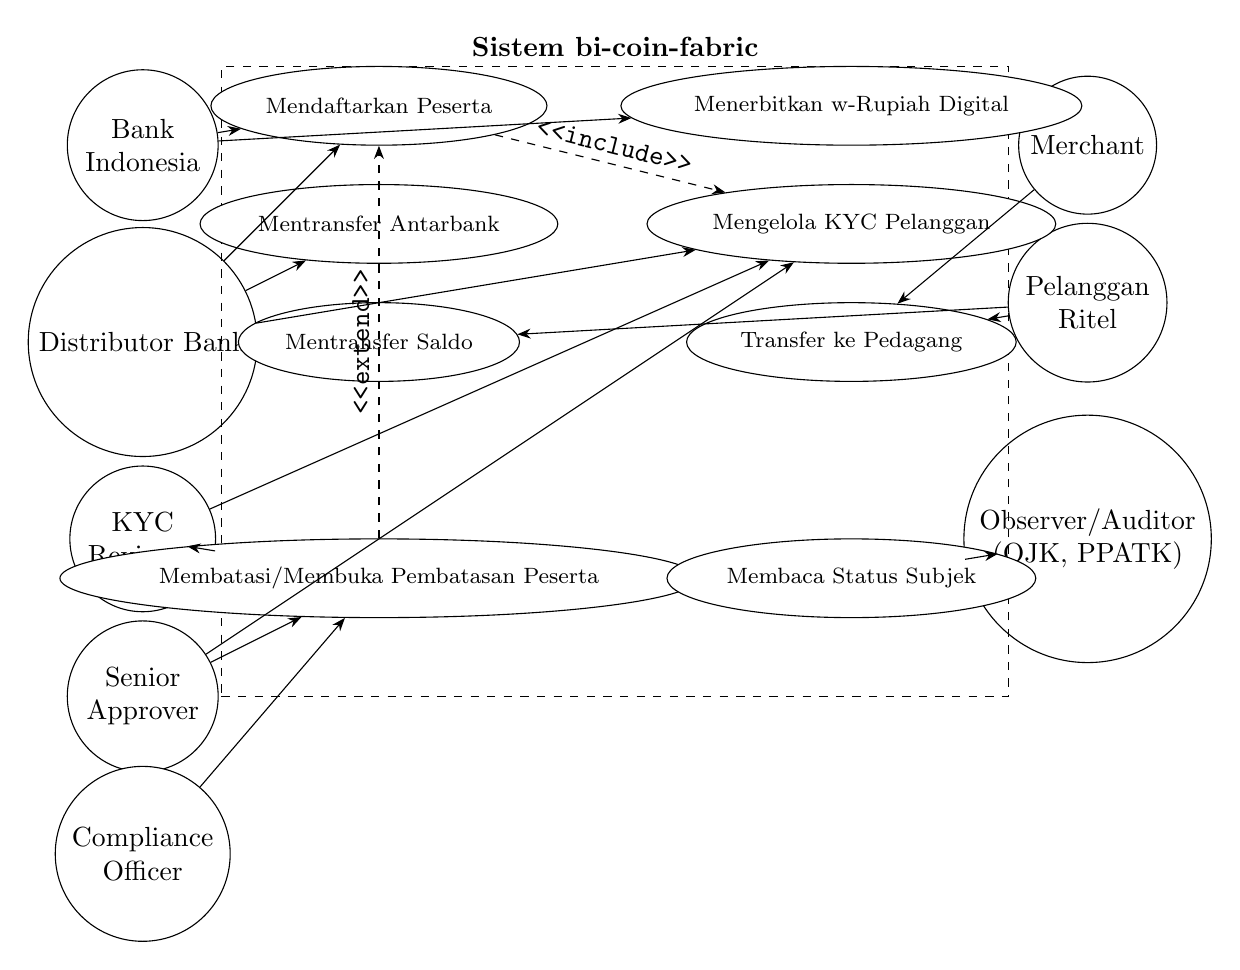
\begin{tikzpicture}[node distance=1.5cm]

\node[actor] (bi) at (0,8) {Bank\\Indonesia};
\node[actor] (db) at (0,5.5) {Distributor Bank};
\node[actor] (kyc) at (0,3) {KYC\\Reviewer};
\node[actor] (sa) at (0,1) {Senior\\Approver};
\node[actor] (co) at (0,-1) {Compliance\\Officer};
\node[actor] (m) at (12,8) {Merchant};
\node[actor] (pr) at (12,6) {Pelanggan\\Ritel};
\node[actor] (obs) at (12,3) {Observer/Auditor\\(OJK, PPATK)};

\node[system, label=above:{\textbf{Sistem bi-coin-fabric}}] (sys) at (6,5) {};

\node[usecase] (uc1) at (3,8.5) {Mendaftarkan Peserta};
\node[usecase] (uc2) at (9,8.5) {Menerbitkan w-Rupiah Digital};
\node[usecase] (uc3) at (3,7) {Mentransfer Antarbank};
\node[usecase] (uc4) at (9,7) {Mengelola KYC Pelanggan};
\node[usecase] (uc5) at (3,5.5) {Mentransfer Saldo};
\node[usecase] (uc6) at (9,5.5) {Transfer ke Pedagang};
\node[usecase] (uc8) at (3,2.5) {Membatasi/Membuka Pembatasan Peserta};
\node[usecase] (uc10) at (9,2.5) {Membaca Status Subjek};

\draw[association] (bi) -- (uc1);
\draw[association] (bi) -- (uc2);
\draw[association] (db) -- (uc3);
\draw[association] (kyc) -- (uc8);
\draw[association] (sa) -- (uc8);
\draw[association] (db) -- (uc1);
\draw[association] (db) -- (uc4);
\draw[association] (kyc) -- (uc4);
\draw[association] (sa) -- (uc4);
\draw[association] (co) -- (uc8);
\draw[association] (m) -- (uc6);
\draw[association] (pr) -- (uc5);
\draw[association] (pr) -- (uc6);
\draw[association] (obs) -- (uc10);

\draw[dependency] (uc1) -- (uc4) node[midway, above, sloped] {\texttt{<<include>>}};
\draw[dependency] (uc8) -- (uc1) node[midway, above, sloped] {\texttt{<<extend>>}};

\end{tikzpicture}
\end{figure}

\clearpage

\section*{UC02 — Operasi Institusional (Institutional Operations)}

\begin{figure}[H]
\centering
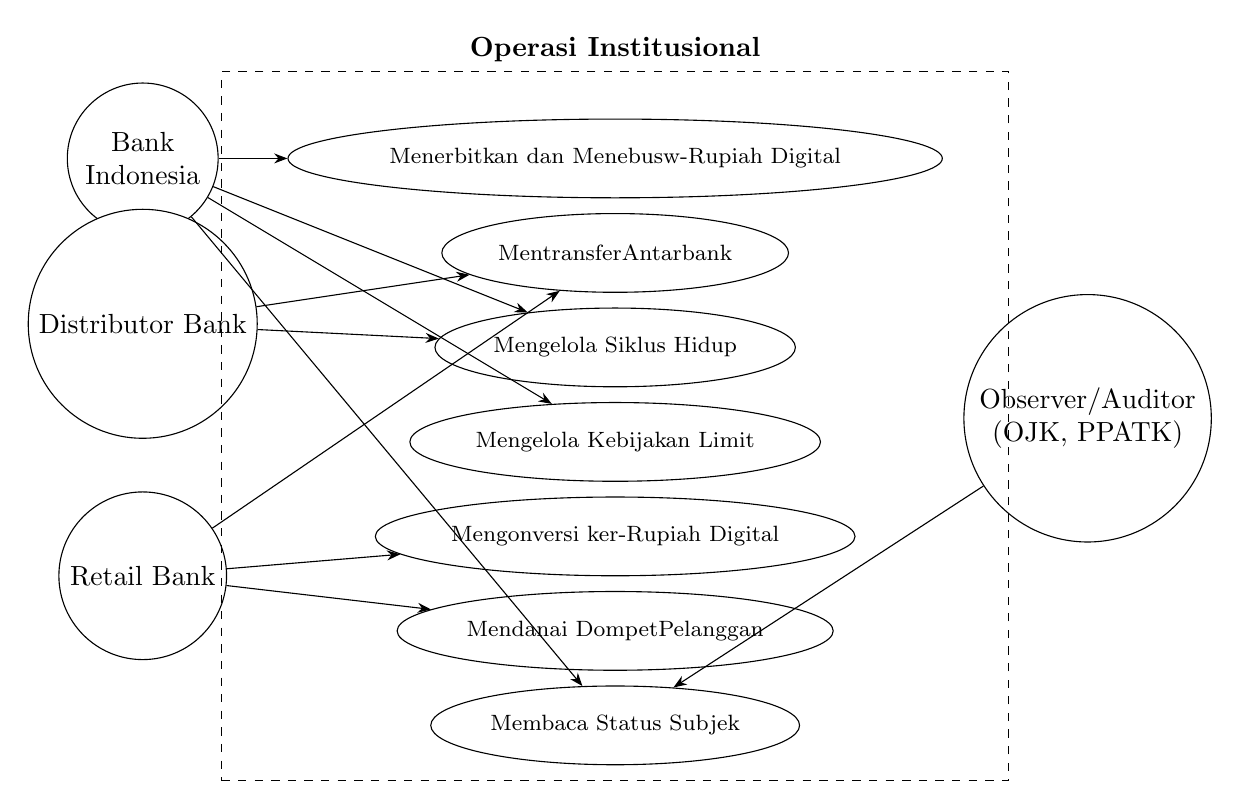
\begin{tikzpicture}[node distance=1.5cm]

\node[actor] (bi) at (0,6.3) {Bank\\Indonesia};
\node[actor] (db) at (0,4.2) {Distributor Bank};
\node[actor] (rb) at (0,1.0) {Retail Bank};
\node[actor] (obs) at (12,3.0) {Observer/Auditor\\(OJK, PPATK)};

\node[system, minimum height=9cm, label=above:{\textbf{Operasi Institusional}}] (sys) at (6,2.9) {};

\node[usecase] (uc1) at (6,6.3) {Menerbitkan dan Menebus\\w-Rupiah Digital};
\node[usecase] (uc2) at (6,5.1) {Mentransfer\\Antarbank};
\node[usecase] (uc3) at (6,3.9) {Mengelola Siklus Hidup};
\node[usecase] (uc4) at (6,2.7) {Mengelola Kebijakan Limit};
\node[usecase] (uc5) at (6,1.5) {Mengonversi ke\\r-Rupiah Digital};
\node[usecase] (uc6) at (6,0.3) {Mendanai Dompet\\Pelanggan};
\node[usecase] (uc7) at (6,-0.9) {Membaca Status Subjek};

\draw[association] (bi) -- (uc1);
\draw[association] (bi) -- (uc3);
\draw[association] (bi) -- (uc4);
\draw[association] (bi) -- (uc7);
\draw[association] (db) -- (uc2);
\draw[association] (db) -- (uc3);
\draw[association] (rb) -- (uc2);
\draw[association] (rb) -- (uc5);
\draw[association] (rb) -- (uc6);
\draw[association] (obs) -- (uc7);

\end{tikzpicture}
\end{figure}

\clearpage

\section*{UC03 — Operasi Retail (Retail Operations)}

\begin{figure}[H]
\centering
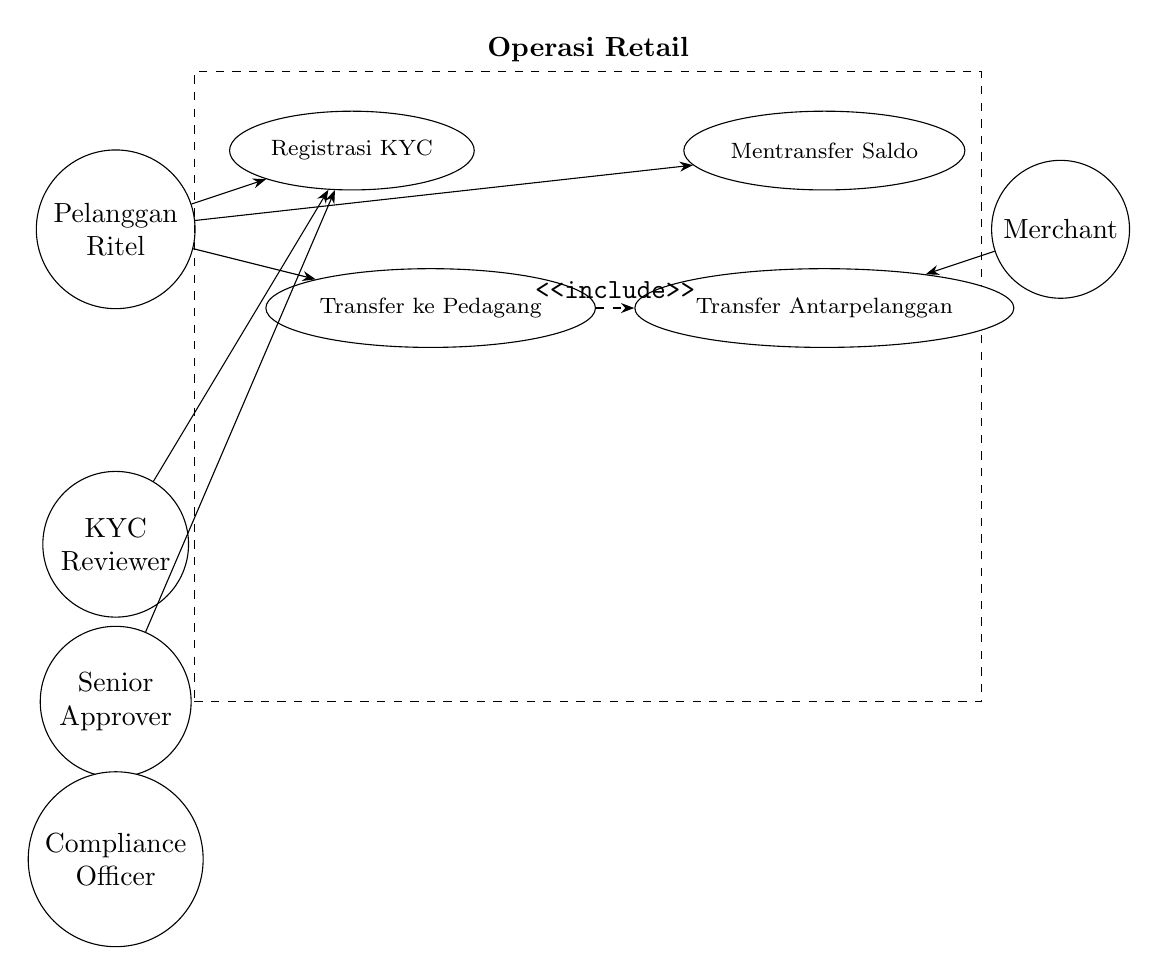
\begin{tikzpicture}[node distance=1.5cm]

\node[actor] (pr) at (0,6) {Pelanggan\\Ritel};
\node[actor] (m) at (12,6) {Merchant};
\node[actor] (kyc) at (0,2) {KYC\\Reviewer};
\node[actor] (sa) at (0,0) {Senior\\Approver};
\node[actor] (co) at (0,-2) {Compliance\\Officer};

\node[system, label=above:{\textbf{Operasi Retail}}] (sys) at (6,4) {};

\node[usecase] (uc1) at (3,7) {Registrasi KYC};
\node[usecase] (uc2) at (9,7) {Mentransfer Saldo};
\node[usecase] (uc3) at (9,5) {Transfer Antarpelanggan};
\node[usecase] (uc4) at (4,5) {Transfer ke Pedagang};

\draw[association] (pr) -- (uc1);
\draw[association] (pr) -- (uc2);
\draw[association] (pr) -- (uc4);
\draw[association] (m) -- (uc3);
\draw[association] (kyc) -- (uc1);
\draw[association] (sa) -- (uc1);

\draw[dependency] (uc4) -- (uc3) node[midway, above, sloped] {\texttt{<<include>>}};

\end{tikzpicture}
\end{figure}

\end{document}
